% !TeX TXS-program:compile = txs:///pdflatex/[--shell-escape]
\documentclass[10pt,landscape,a4paper]{article}
\usepackage[normalem]{ulem}
\usepackage{tikz}
\usetikzlibrary{shapes,positioning,arrows,fit,calc,graphs,graphs.standard}
\usepackage[nosf]{kpfonts}
\usepackage[t1]{sourcesanspro}
\usepackage{multicol}
\usepackage{wrapfig}
\usepackage[top=0mm,bottom=0mm,left=0mm,right=1mm]{geometry}
\usepackage[framemethod=tikz]{mdframed}
\usepackage{microtype}
\usepackage{tabularx}
\usepackage{array}
\usepackage{hhline}
\usepackage{makecell}
\usepackage{mathtools}
\usepackage{xcolor}
\usepackage{graphicx}
\usepackage{listings}
\usepackage{mips}
\lstset{language=[mips]Assembler}

\DeclarePairedDelimiter{\ceil}{\lceil}{\rceil}

\newcommand\codeblue[1]{\textcolor{blue}{\code{#1}}}

\usepackage{lastpage}
\usepackage{datetime}
\yyyymmdddate
\renewcommand{\dateseparator}{-}
\let\bar\overline

\definecolor{myblue}{cmyk}{1,.72,0,.38}

\def\firstcircle{(0,0) circle (1.5cm)}
\def\secondcircle{(0:2cm) circle (1.5cm)}

\colorlet{circle edge}{myblue}
\colorlet{circle area}{myblue!5}

\tikzset{filled/.style={fill=circle area, draw=circle edge, thick},
    outline/.style={draw=circle edge, thick}}

\pgfdeclarelayer{background}
\pgfsetlayers{background,main}
\graphicspath{{.}}

\renewcommand{\baselinestretch}{.8}
\pagestyle{empty}
%\usepackage{chngcntr}

\usepackage{verbatim}

\usepackage{etoolbox}
\makeatletter
\preto{\@verbatim}{\topsep=0pt \partopsep=0pt }
\makeatother

\counterwithin*{equation}{section}
\counterwithin*{equation}{subsection}
\usepackage{enumitem}
\newlist{legal}{enumerate}{10}
\setlist[legal]{label*=\arabic*.,leftmargin=2.5mm}
\setlist[itemize]{leftmargin=3mm}
\setlist{nosep}
\usepackage[cache=false]{minted}

\def\code#1{\texttt{#1}}

\newenvironment{descitemize} % a mixture of description and itemize
{\begin{description}[leftmargin=*,before=\let\makelabel\descitemlabel]}
{\end{description}}

\newcommand{\descitemlabel}[1]{%
\textbullet\ \textbf{#1}%
}
\makeatletter

\renewcommand{\section}{\@startsection{section}{1}{0mm}%
                                {.2ex}%
                                {.2ex}%x
                                {\color{myblue}\sffamily\small\bfseries}}
\renewcommand{\subsection}{\@startsection{subsection}{1}{0mm}%
                                {.2ex}%
                                {.2ex}%x
                                {\sffamily\bfseries}}
\renewcommand{\subsubsection}{\@startsection{subsubsection}{1}{0mm}%
                                {.2ex}%
                                {.2ex}%x
                                {\rmfamily\bfseries}}

\def\mathcolor#1#{\@mathcolor{#1}}
\def\@mathcolor#1#2#3{%
  \protect\leavevmode
  \begingroup
  \color#1{#2}#3%
  \endgroup
}

\makeatother
\setlength{\parindent}{0pt}

\setminted{tabsize=2, breaklines}
% Remove belowskip of minted
\setlength\partopsep{-\topsep}


\newcolumntype{a}{>{\hsize=1.5\hsize}X}
\newcolumntype{b}{>{\hsize=.25\hsize}X}

\setlength\columnsep{1.5pt}
\setlength\columnseprule{0.1pt}
\begin{document}
\setlength{\abovedisplayskip}{0pt}
\setlength{\belowdisplayskip}{0pt}

\scriptsize
\begin{multicols*}{3}
  \section{C Programming Language}
  \subsection{Data Types}
  \begin{tabularx}{\columnwidth}{|b|b|a|}
    \hline
    \textbf{Type}   & \textbf{\texttt{sizeof}} & \textbf{range}                                               \\
    \hline
    \texttt{int}    & 4 bytes                  & \makecell[l]{2s complement, thus $(-2^{31})$ to $(2^{31}-1)$ \\ OR (-2,147,483,648 to 2,147,483,647)} \\ \hline
    \texttt{float}  & 4 bytes                  & 1-bit sign, 8-bit exponent (excess-127), 23-bit mantissa     \\ \hline
    \texttt{double} & 8 bytes                  & 1-bit sign, 11-bit exponent (excess-1023), 52-bit mantissa   \\ \hline
    \texttt{char}   & 1 byte                   & ASCII (7 bits + 1 parity bit), A is 100 0001                 \\ \hline
  \end{tabularx}
  Note that for mantissa there is an implicit leading bit 1
  \subsection{Format Specifiers}
  \begin{tabular}{|l|l|l|}
    \hline
                 & \textbf{Type}                  & \textbf{fn}           \\
    \hline
    \texttt{\%c} & \texttt{char}                  & \texttt{printf/scanf} \\ \hline
    \texttt{\%d} & \texttt{int}                  & \texttt{printf/scanf} \\ \hline
    \texttt{\%f} & \texttt{float}/\texttt{double} & \texttt{printf}       \\ \hline
  \end{tabular}
  \begin{tabular}{|l|l|l|}
    \hline
                  & \textbf{Type}   & \textbf{fn}     \\
    \hline
    \texttt{\%f}  & \texttt{float}  & \texttt{scanf}  \\ \hline
    \texttt{\%lf} & \texttt{double} & \texttt{scanf}  \\ \hline
    \texttt{\%p}  & pointers        & \texttt{printf} \\ \hline
  \end{tabular}
  \subsection{Escape Sequences}
  \begin{tabular}{|l|l|}
    \hline
                              & \textbf{Meaning} \\
    \hline
    \texttt{\textbackslash n} & new line         \\ \hline
    \texttt{\textbackslash t} & tab              \\ \hline
  \end{tabular}
  \begin{tabular}{|l|l|}
    \hline
                              & \textbf{Meaning} \\
    \hline
    \texttt{\textbackslash "} & double-quote "   \\ \hline
    \texttt{\%\%}             & percent \%       \\ \hline
  \end{tabular}
  \section{Numbering Systems}
  \subsection{Data Representation}
  \begin{itemize}
    \item 1 byte = 8 bits, 1 nibble = 4 bits
    \item 1 word = Multiple of bytes (usually in powers of 2)
    \item $n$ bits can represent up to $2^n$ values. Thus, to present $m$ values, $\ceil{\log_2m}$ is required
  \end{itemize}
  \subsection{Decimal to Binary Conversion}
  \begin{itemize}
    \item For whole numbers: repeated division-by-2 (look at remainder, $1^{st}$ digit LSB)
    \item For fractions: repeated multiplication-by-2 (look at "quotient", $1^{st}$ digit MSB)
  \end{itemize}
  \subsection{Representation of Signed Binary Numbers}
  \newcolumntype{c}{>{\hsize=0.45\hsize}X}
  \newcolumntype{d}{>{\hsize=0.6\hsize}X}
  \newcolumntype{e}{>{\hsize=0.55\hsize}X}
  \newcolumntype{f}{>{\hsize=0.4\hsize}X}
  \begin{tabularx}{\columnwidth}{|c|d|e|f|}
    \hline
                       & Negation                          & Range                             & Zeroes                  \\
    \hline
    Sign-and-Magnitude & invert the sign bit (leading bit) & $-(2^{n-1} - 1)$ to $2^{n-1} - 1$ & $+0_{10}$ and $-0_{10}$ \\ \hline
    1s Complement      & invert all the bits               & $-(2^{n-1} - 1)$ to $2^{n-1} - 1$ & $+0_{10}$ and $-0_{10}$ \\ \hline
    2s Complement      & invert all the bits, then add 1   & $-2^{n-1}$ to $2^{n-1}-1$         & $+0_{10}$               \\ \hline
  \end{tabularx}
  For all of the above, the MSB (Most Significant Bit) represents sign.
  \subsubsection{Sign-and-Magnitude}
  \begin{itemize}
    \item Range (8-bit): $(1111$ $1111)$ to $(0111$ $1111) = -127_{10}$ to $+127_{10}$
    \item Zeroes: $0000$ $0000 = +0_{10}$ and $1000$ $0000 = -0_{10}$
    \item e.g. $(\mathcolor{red}{0}011$ $0100)_{sm} = +011$ $0100_2 = +52_{10}$, $(\mathcolor{red}{1}001$ $0011)_{sm} = -(001$ $0011)_2 = -(19)_{10}$
  \end{itemize}
  \subsubsection{1s Complement (Diminished Radix)}
  \begin{itemize}
    \item Negation: $-x=2^n -x-1$, if given binary: invert all bits
    \item Range (8-bit): $(1000$ $0000)$ to $(0111$ $1111) = -127_{10}$ to $+127_{10}$
    \item Zeroes: $(0000$ $0000) = +0_{10}$ and $(1111$ $1111) = -0_{10}$
    \item e.g. $(0000$ $1110)_{1s} = (0000$ $1110)_2 = (14)_{10}$,
          $(1111$ $0001)_{1s} = -(0000$ $1110)_2 = -(14)_{10}$
  \end{itemize}
  \subsubsection{2s Complement (Radix complement)}
  \begin{itemize}
    \item Negation: $-x = 2^n - x$, if given binary: invert all bits then add 1
    \item Range (8-bit): $(1000$ $0000) = -128_{10}$ to $(0111$ $1111) = +127_{10}$
    \item Zero: $(0000$ $0000) = +0_{10}$
    \item e.g. $(0000$ $1110)_{2s} = (0000$ $1110)_2 = (14)_{10}$,  $(1111$ $0010)_{2s} = -(0000$ $1110)_2 = -(14)_{10}$
  \end{itemize}
  \subsubsection{Excess-k}
  \begin{itemize}
    \item Also known as offset binary. Use 0000 to represent $-k$ (lowest number possible)
    \item For unsigned, with $n$-bit number, $k=2^{n-1}-1$ or $k=2^{n-1}$
  \end{itemize}
  \subsubsection{Comparison}
  \newcolumntype{g}{>{\hsize=0.15\hsize}X}
  \newcolumntype{h}{>{\hsize=0.4\hsize}X}
  \begin{tabularx}{\columnwidth}{|g|h|h|h|h|g|}
    \hline
    \textbf{Value} & \textbf{Sign-and-Magnitude} & \textbf{1s Complement} & \textbf{2s Complement} & \textbf{Excess-8} & \textbf{Value} \\
    \hline
    +7             & 0111                        & 0111                   & 0111                   & 1111              & +7             \\ \hline
    +6             & 0110                        & 0110                   & 0110                   & 1110              & +6             \\ \hline
    +5             & 0101                        & 0101                   & 0101                   & 1101              & +5             \\ \hline
    +4             & 0100                        & 0100                   & 0100                   & 1100              & +4             \\ \hline
    +3             & 0011                        & 0011                   & 0011                   & 1011              & +3             \\ \hline
    +2             & 0010                        & 0010                   & 0010                   & 1010              & +2             \\ \hline
    +1             & 0001                        & 0001                   & 0001                   & 1001              & +1             \\ \hline
    +0             & 0000                        & 0000                   & 0000                   & 1000              & +0             \\ \hline
    -0             & 1000                        & 1111                   & -                      & -                 & -0             \\ \hline
    -1             & 1001                        & 1110                   & 1111                   & 0111              & -1             \\ \hline
    -2             & 1010                        & 1101                   & 1110                   & 0110              & -2             \\ \hline
    -3             & 1011                        & 1100                   & 1101                   & 0101              & -3             \\ \hline
    -4             & 1100                        & 1011                   & 1100                   & 0100              & -4             \\ \hline
    -5             & 1101                        & 1010                   & 1011                   & 0011              & -5             \\ \hline
    -6             & 1110                        & 1001                   & 1010                   & 0010              & -6             \\ \hline
    -7             & 1111                        & 1000                   & 1001                   & 0001              & -7             \\ \hline
    -8             & -                           & -                      & 1000                   & 0000              & -8             \\ \hline
  \end{tabularx}

  \subsection{Operation on binary numbers}
  Algorithm for \textbf{Subtraction}: $A - B = A + (-B)$, do sign extension before complementing\\
  Algorithm for \textbf{Overflow Check}: if MSB of first and second are the same, then MSB of resulting numbers must be the same too.
  \subsubsection{2s Complement on Addition}
  Algorithm: (1) Perform binary addition. (2) Ignore the carry out of the MSB. (3) Check for overflow.
  \begin{verbatim}
Example, 2s Complement 4-bit
+3  0011                -2    1110                -3     1101
+4  0100                -6    1010                -6     1010
--- -----               ---   -----               ---    -----
+7  0111 (No overflow)  -8 (1)1000 (No overflow)  -9  (1)0111 (Overflow!)
\end{verbatim}
  \subsubsection{1s Complement on Addition}
  Algorithm: (1) Perform binary addition. (2) If there is carry out of the MSB, \textcolor{red}{add 1} to the result. (3) Check for overflow.\\
  If doing 1s complement addition on decimals and there is an overflow from MSB, \textcolor{red}{add 1 to LSB of decimal portion}
  \begin{verbatim}
Example, 1s Complement 4-bit
+3  0011                -2    1101                -3     1100
+4  0100                -5    1010                -6     1001
--- -----               ---   -----               ---    -----
+7  0111 (No overflow)  -7 (1)0111                -9  (1)0101
                                 1                          1
                              -----                      -----
                              1000 (No overflow)         0110 (Overflow!)
\end{verbatim}
  \subsection{Floating Point}
  \begin{itemize}
    \item Single precision 32 bits: 1-bit sign, 8-bit exponent (excess-127), 23-bit mantissa
    \item Double precision 64 bits: 1-bit sign, 11-bit exponent (excess-1023), 52-bit mantissa
    \item e.g. $-6.5_{10} = -110.1_{2} = -1.101_{2} \times 2^2$, Exponent (excess-127) $= 2 + 127 = 129 = 1000$ $0001_2$
  \end{itemize}

  \begin{verbatim}
Sign Exponent          Mantissa
 1   10000001 10100000000000000000000
\end{verbatim}
  Hence, $1100$ $0000$ $1101$ $0000$ $0000$ $0000$ $0000$ $0000_2 = C0D0 0000_{16}$\\
  (as \texttt{float}$ = -6.5$, as \texttt{int}$ = -1,060,110,336$)
  \section{Pointers and Functions}
  \subsection{Pointers}
  \begin{itemize}
    \item Convention: \mintinline{C}{int *abc;} AND \mintinline{C}{void f(int *);}
    \item $\%p$ used as format modifier for addresses and is printed out in \textcolor{red}{hexadecimal}
    \item When we do \mintinline{C}{ptr++}, it increases the address by the size of the datatype
  \end{itemize}
  \subsection{Functions}
  \begin{itemize}
    \item Function prototype (just the type of its parameters): e.g. \mintinline{C}{void g(int, int);}
    \item Without function prototypes, compiler assumes default return type of \mintinline{C}{int}
  \end{itemize}
  \section{Arrays, Strings, Structures}
  \subsection{Arrays}
  \begin{itemize}
    \item When initialised with fewer values than elements, the rest are initialised as 0 (for \mintinline{C}{int}).
    \item When an array name appears in an expression or passed as a parameter to a function, it refers to the address of the first element (i.e \mintinline{C}{&a[0]})
    \item \mintinline{C}{int source[5]; int dest[5]; source = dest} is \textcolor{red}{illegal}!
  \end{itemize}
  \subsection{String}
  \begin{itemize}
    \item An array of characters, terminated by a null character \mintinline{C}{'\0'} (ASCII value: 0	)
    \item Initialising: \mintinline{C}{char str[4] = "egg";} or \mintinline{C}{char str[4] = {'e', 'g', 'g', '\0'};}
    \item Read from stdin: \mintinline{C}{fgets(str, size, stdin); // reads until (size - 1) or '\n'} and \mintinline{C}{scanf("%s", str); // reads until whitespace}
      \\(note that \mintinline{C}{fgets} also reads in \mintinline{C}{'\n'} and we may need to replace it with \mintinline{C}{'\0'} if necessary (Lect 5, Slide 21))
    \item Print to stdout: \mintinline{C}{puts(str);} which is equivalent to \mintinline{C}{printf("%s\n", str)}
    \item String functions:
          \begin{itemize}
            \item \mintinline{C}{strlen(s)}: returns the no of chars in \mintinline{C}{s}
            \item \mintinline{C}{strcmp(s1, s2)}: compare ASCII values of corresponding characters, returns $\mathbb{Z}^+$ if s1 is lexographically greater, $0$ if equal, $\mathbb{Z}^-$ otherwise
            \item \mintinline{C}{strncmp(s1, s2, n)}: compare first $n$ chars of s1 and s2
            \item \mintinline{C}{strcpy(s1, s2)}: copy the string pointed by s2 into array pointed by s1, returns s1. E.g. \mintinline{C}{char s[4]; strcpy(s, "asdfgh"); // s == {'a', 's', 'd', '\0'};}
            \item \mintinline{C}{strncpt(s1, s2, n)}: copy the first $n$ chars of string pointed by s2 to s1
          \end{itemize}
  \end{itemize}
  \subsection{Structures}
  \begin{itemize}
    \item Structures allow grouping of heterogeneous members of different types.
    \item Assignment  \mintinline{C}{result2 = result1;} copies the entire structure.
    \item Passing structure to function: the entire structure is copied, original structure is not modified by function
    \item Alternatively, to change original structure, one can use pointer. Syntactic sugar: \mintinline{C}{(*player_ptr).name == player_ptr->name;}
    \item E.g.: \begin{minted}{C}
typedef struct {
  int day, month, year;
} date_t;
typedef struct {
  int stuNum;
  date_t birthday;
} student_t;
student_t s1 = {1049858, {31, 12, 2020}}; // s1.birthday.month == 12
  \end{minted}
  \end{itemize}
  \section{C for Hardware Programming}
  \subsection{Code Compilation Process}
  C Program (.c) -> \textbf{Preprocessor} -> Preprocessed code (.i) -> \textbf{Compiler} -> Assembly code (.asm) -> \textbf{Assembler} -> Object code (.o) -> \textbf{Linker} -> Executable (.hex)
  \section{MIPS}
  \subsection{Loading a 32-bit constant into a register}
  \begin{enumerate}
    \item Use \texttt{lui} to set the upper 16-bit: \lstinline|lui \$t0, 0xAAAA|. Note that \lstinline|lui| sets the lower 16 bits to 0 automatically
    \item Use \texttt{ori} to set the lower-order bits: \lstinline|ori $t0, $t0, 0xF0F0|
  \end{enumerate}
  \subsection{Memory Organisation}
  \begin{itemize}
    \item Each address contains 1 byte = 8 bit of content.
    \item Memory addresses are 32-bit long ($2^{30}$ memory words).
    \item 32 registers, each 4-byte long. Each word is also 4-byte long. (Note that words are usually $2^n$ bytes)
  \end{itemize}
  \subsection{MIPS Instruction Classification}
  \subsubsection{R-format}
  \begin{itemize}
    \item \texttt{op \$rd, \$rs, \$rt}
    \item \texttt{sll \$rd, \$rt, shamt} (rs = 0)
  \end{itemize}
  \subsubsection{I-format}
  \begin{itemize}
    \item \texttt{op \$rt, \$rs, Immediate}
    \item Immediate is a \textcolor{red}{16 bit 2s complement} constant
    \item Displacement address: offset from address in rs
    \item PC-relative address: no of instructions from next instruction $PC = PC + 4 + (Immediate \times 4)$
  \end{itemize}
  \subsubsection{J-format (can jump up to 256MB range)}
  \begin{itemize}
    \item \texttt{op Immediate}
    \item pseudo-direct address: remove last 2 bit (since word-aligned, by default the 2 least significant bits are 00) and 4 most significant bits (always the same as instruction address).
    \item eg \texttt{xxxx00001111000011110000111100\sout{00}}, immediate is \texttt{00001111000011110000111100}
  \end{itemize}
  \section{Instruction Set Architecture}
  For modern processors: \textbf{General-Purpose Register} (GPR) is most common. \textbf{RISC} typically uses \textbf{Register-Register (Load/Store)} design, e.g. MIPS, ARM. \textbf{CISC} use a mixture of Register-Register and Register-Memory, e.g. IA32
  \subsection{Data Storage}
  \begin{descitemize}
    \item [Stack architecture]: Operands are implicitly on top of the stack.
    \item [Accumulator architecture]: One operand is implicitly in the accumulator (a special register)
    \item [General-purpose register architecture]: only explicit operands
    \begin{descitemize}
      \item [Register-memory architecture]: one operand in memory.
      \item [Register-register (or load store) architecture]
    \end{descitemize}
    \item [Memory-memory architecture]: all operands in memory.
  \end{descitemize}
  \subsection{Memory Addressing Modes}
  \begin{descitemize}
    \item [Endianness]: Relative ordering of bytes in a multiple-byte word stored in memory
    \begin{descitemize}
      \item [Big-endian]: \textbf{Most} significant byte stored in lowest address
      \item [Little-endian]: \textbf{Least} significant byte stored in lowest address ("reverse-order")
    \end{descitemize}
    \item [Addressing modes]: in MIPS, only 3: \textbf{Register} \lstinline|add $t1, $t2, $t3|, \textbf{Immediate} \lstinline|addi $t1, $t2, 98|, \textbf{Displacement} \lstinline|lw $t1, 20($t2)|
  \end{descitemize}
  \subsection{Operations in the instruction set}
  Amdahl's law: make common cases fast. Optimise frequently used instructions (\textbf{Load}: 22\%, \textbf{Conditional Branch}: 20\%, \textbf{Compare} 16\%, \textbf{Store}: 12\%)
  \subsection{Instruction Formats}
  \begin{descitemize}
    \item [Instruction Length]:
    \begin{descitemize}
      \item [Variable-length instructions]: Require multi-step fetch and decode. Allow for a more flexible (but complex) and compact instruction set.
      \item [Fixed-length instructions]: used in most RISC, e.g. MIPS instructions are 4-bytes long. Allow for easy fetch and decode, simplify pipelining and parallelism. Instruction bits are scarce.
      \item [Hybrid instructions]: a mix of variable- and fixed-length instructions.
    \end{descitemize}
    \item [Instruction Fields]: \textbf{opcode} (unique code to specify the desired operation) and \textbf{operands} (zero or more additional information needed for the operation)
  \end{descitemize}
  \subsection{Encoding the Instruction Set}
  \begin{descitemize}
    \item [Expanding Opcode] scheme:
    \begin{descitemize}
      \item E.g. \textbf{Type-A}: \textbf{6-bit} opcode, \textbf{Type-B}: \textbf{11-bits} opcode. Max no of instructions = $1 + (2^6 - 1)\times 2^5 = 2017$\\
      (1 Type-A instruction, Type-B "steals" [$2^6-1$] opcodes from Type-A to prefix, each prefix having [$2^{11-6} = 2^5$] opcodes)
    \end{descitemize}
  \end{descitemize}
  \section{Datapath}
  \subsection{Instruction Execution Cycle}
  For MIPS: (1)Fetch (2)Decode \& Operand Fetch (3)ALU (4)Memory Access (5)Result Write
  \begin{descitemize}
    \item [Fetch]: Get instruction from memory, address is in Program Counter (PC) Register
    \item [Decode]: Find out the operation required
    \item [Operand Fetch]: Get operand(s) needed for operation
    \item [Execute]: Perform the required operation
    \item [Result Write (Store)]: Store the result of the operation
  \end{descitemize}
  \subsection{Elements}
  \begin{descitemize}
    \item [Adder] \textbf{Input}: two 32-bit numbers, \textbf{Output}: sum of input numbers
    \item [Register File] \textbf{Input}: three 5-bit: Read register 1, Read register 2, Write register; 32-bit Write data, \textbf{Output}: two 32-bit Read data 1, Read data 2; \textbf{Control}: 1-bit RegWrite (1 = write)
    \item [Multiplexer] \textbf{Input}: $n$ lines of same width, \textbf{Control}: $m$ bits where $n=2^m$, \textbf{Output}: Select $i^{th}$ input line if control = $i$
    \item [Arithmetic Logic Unit]: \textbf{Input}: two 32-bit numbers, \textbf{Control}: 4-bit to decide the particular operation, \textbf{Output}: 32-bit ALU result, 1-bit isZero? \\
    \begin{tabular}{|l|l|}
      \hline
      \textbf{ALUcontrol} & \textbf{Function} \\ \hline
      \texttt{0000}       & AND               \\
      \texttt{0001}       & OR                \\
      \texttt{0010}       & add               \\
      \hline
    \end{tabular}
    \begin{tabular}{|l|l|}
      \hline
      \textbf{ALUcontrol} & \textbf{Function} \\ \hline
      \texttt{0110}       & subtract          \\
      \texttt{0111}       & slt               \\
      \texttt{1100}       & NOR               \\
      \hline
    \end{tabular}
    \item [Data Memory] \textbf{Input}: 32-bit memory address, 32-bit write data; \textbf{Control}: 1-bit MemWrite, 1-bit MemRead; \textbf{Output}: 32-bit ReadData
    \\
  \end{descitemize}

\section{Useful MIPS commands}
\begin{descitemize}
    \item To get a \textbf{NOT} operation: \lstinline|nor $t0, $t0 $zero| OR \lstinline|xor $t0, $t0 $t2| where \lstinline|$t2| has parity 1 for all its bits
    \item To get a Branch if less than or equal (i.e \lstinline|BLE $s1, $s2, target|) can use \lstinline|slt $t1 $s2 $s1 -> beq $t1, $zero, target| OR\\ \lstinline|sub $t1, $t2, $s1 -> slt $t2, $t1, $zero -> beq $t2, $zero, target|
    \\\\
\end{descitemize}

\textbf{Order of precedence}\\
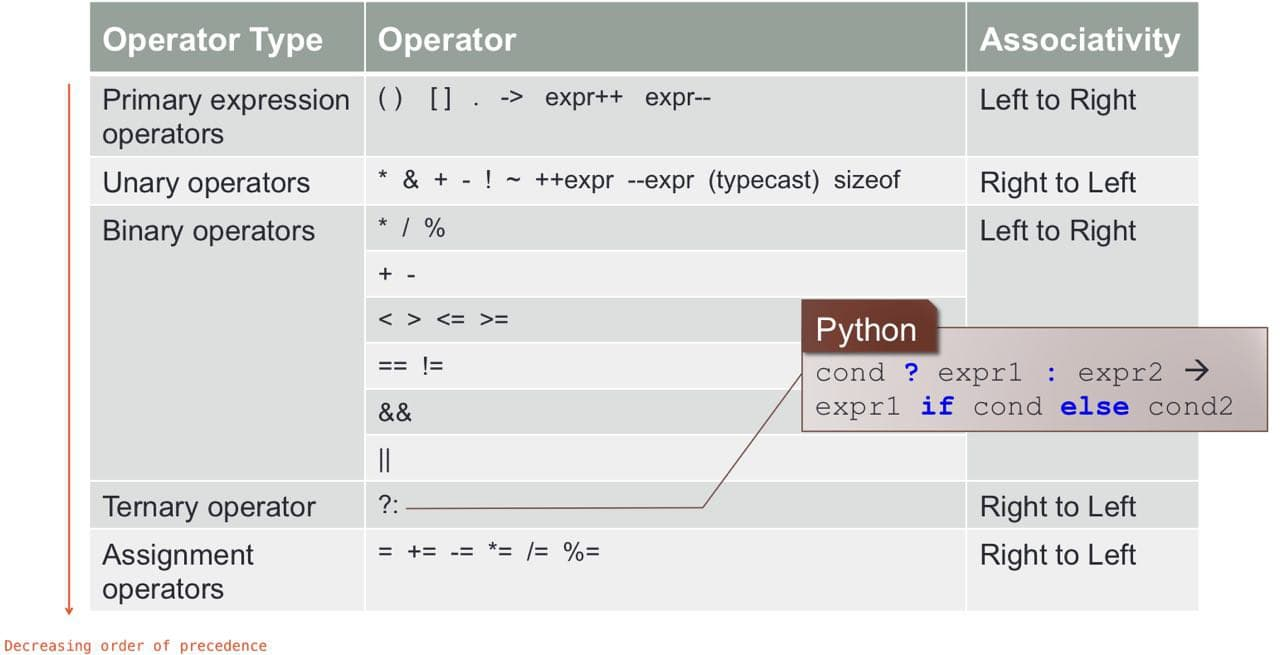
\includegraphics[scale=0.22]{order_of_precedence.jpg}\\\\
\textbf{ALU Control}\\
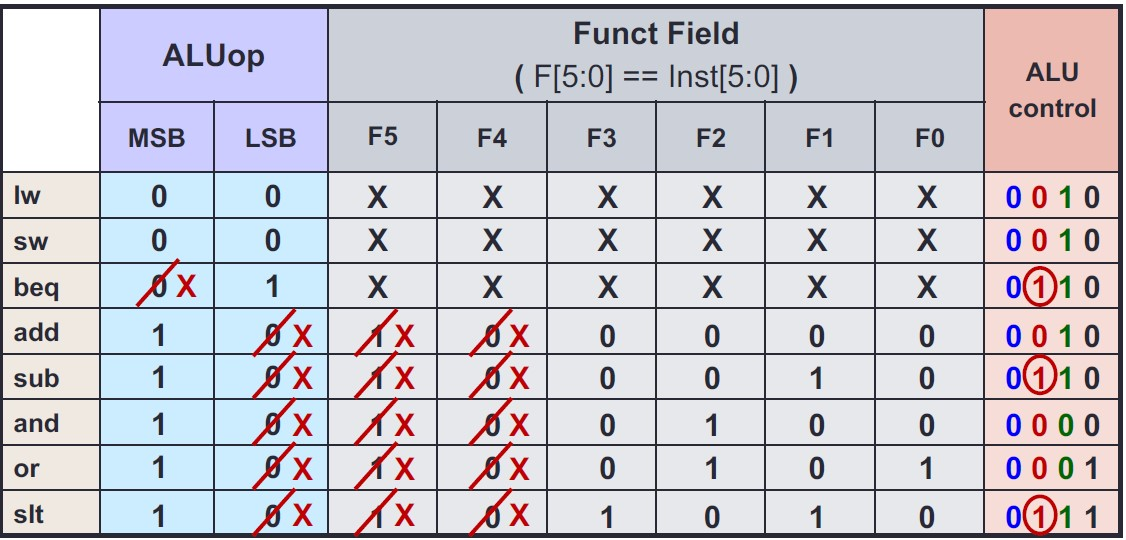
\includegraphics[scale=0.36]{alucontrol.jpg}\\\\
\textbf{Control Signal Output}\\
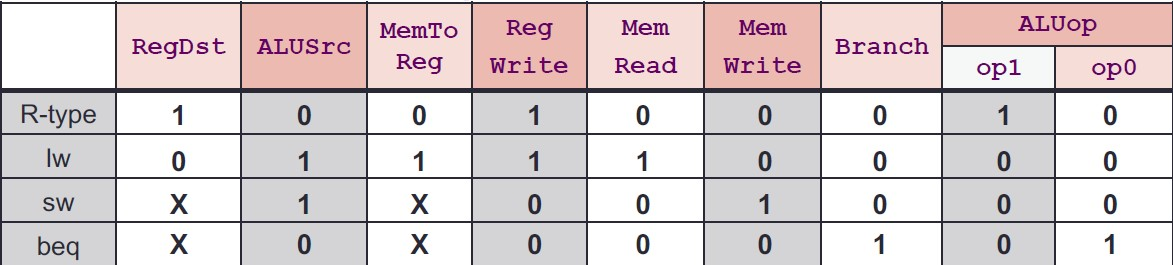
\includegraphics[scale=0.35]{control_signal_output.jpg}
\textbf{Complete Data Path}\\
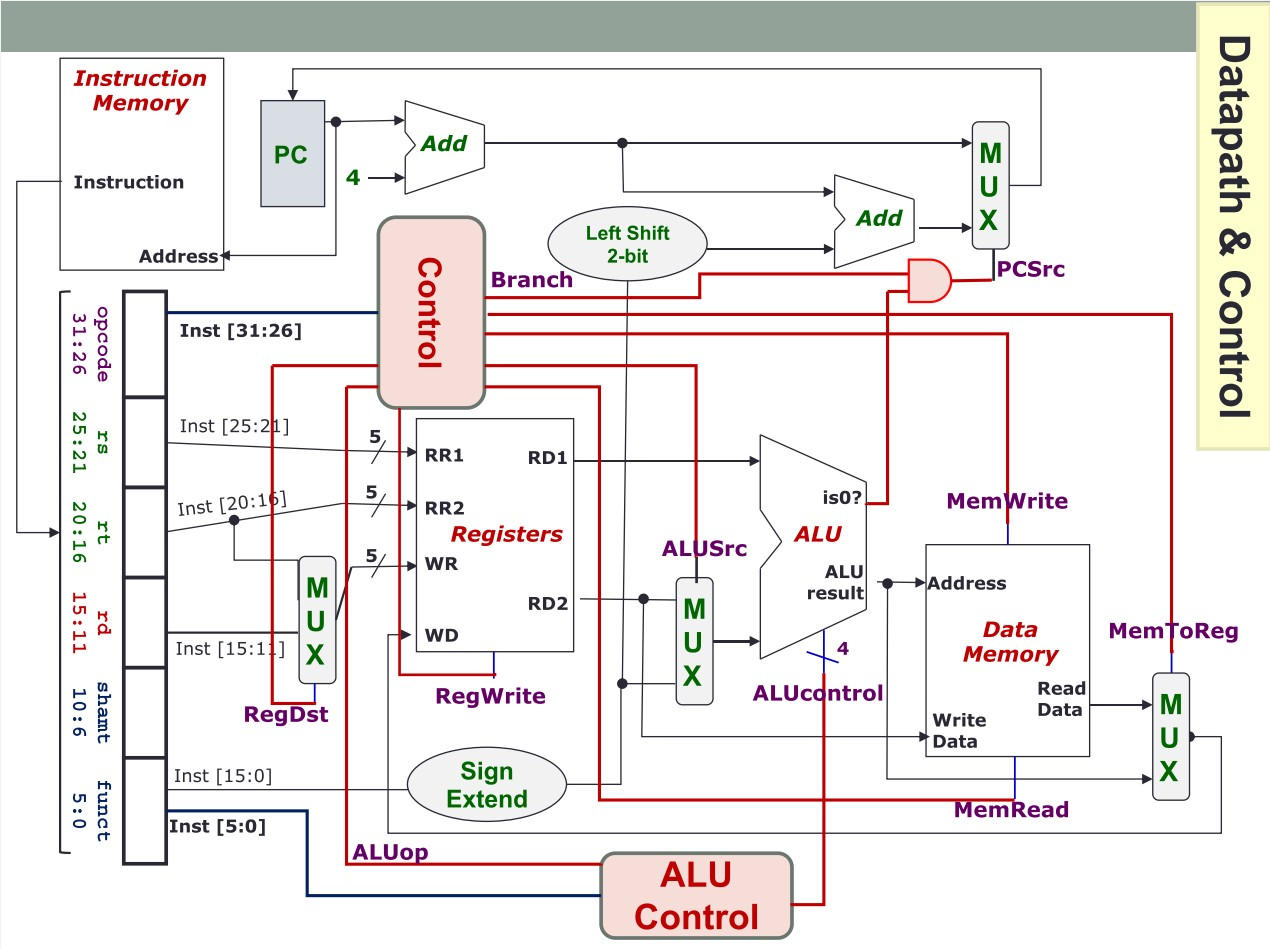
\includegraphics[scale=0.32]{datapath.jpg}\\\\
\textbf{j and jr instruction datapath}\\
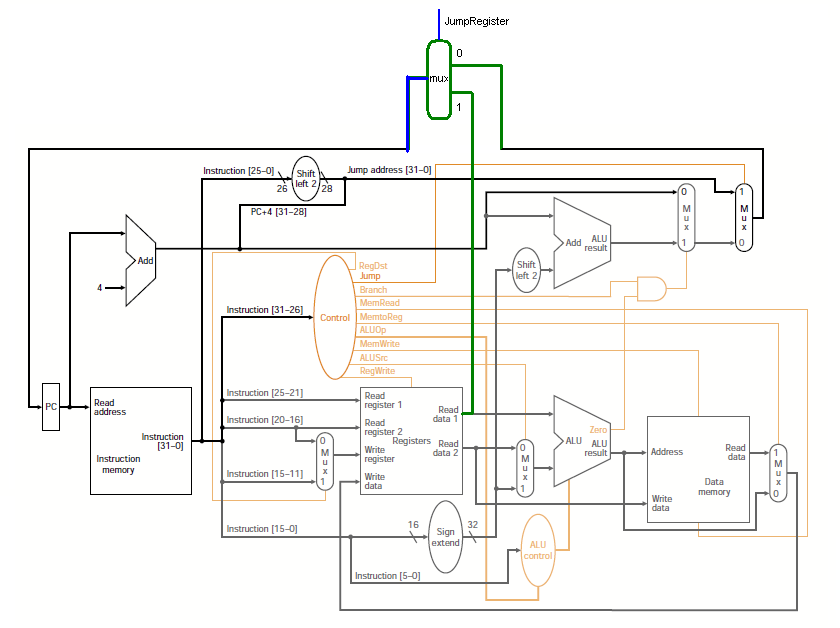
\includegraphics[scale=0.34]{j_instr.png}\\\\
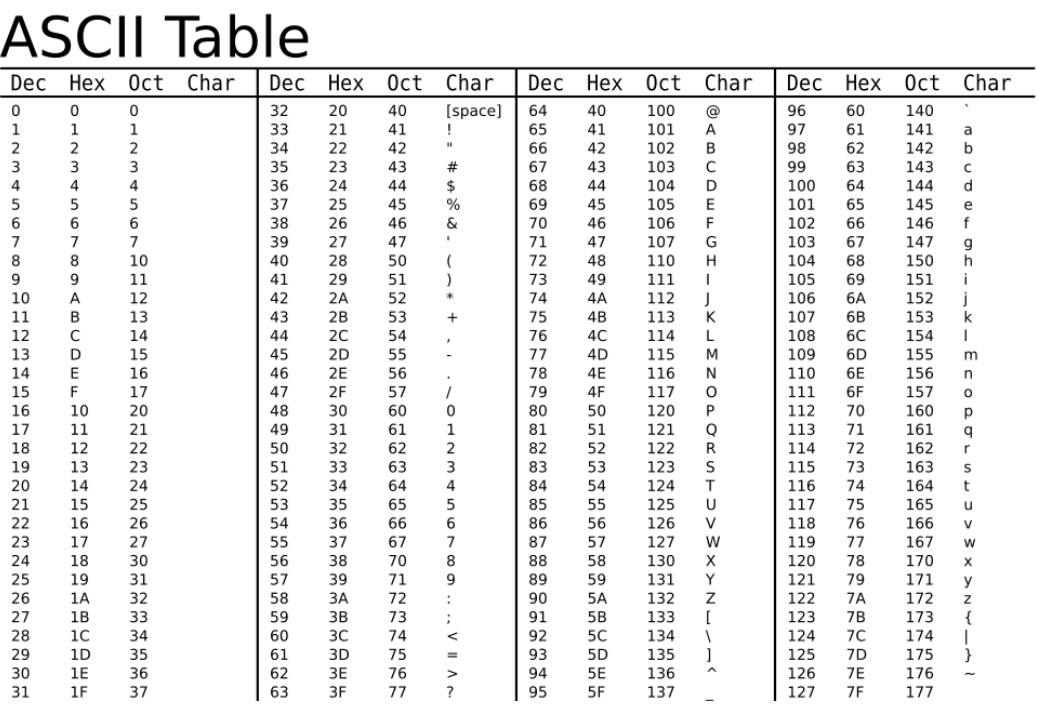
\includegraphics[scale=0.4]{ascii.jpg}
\begin{center}
    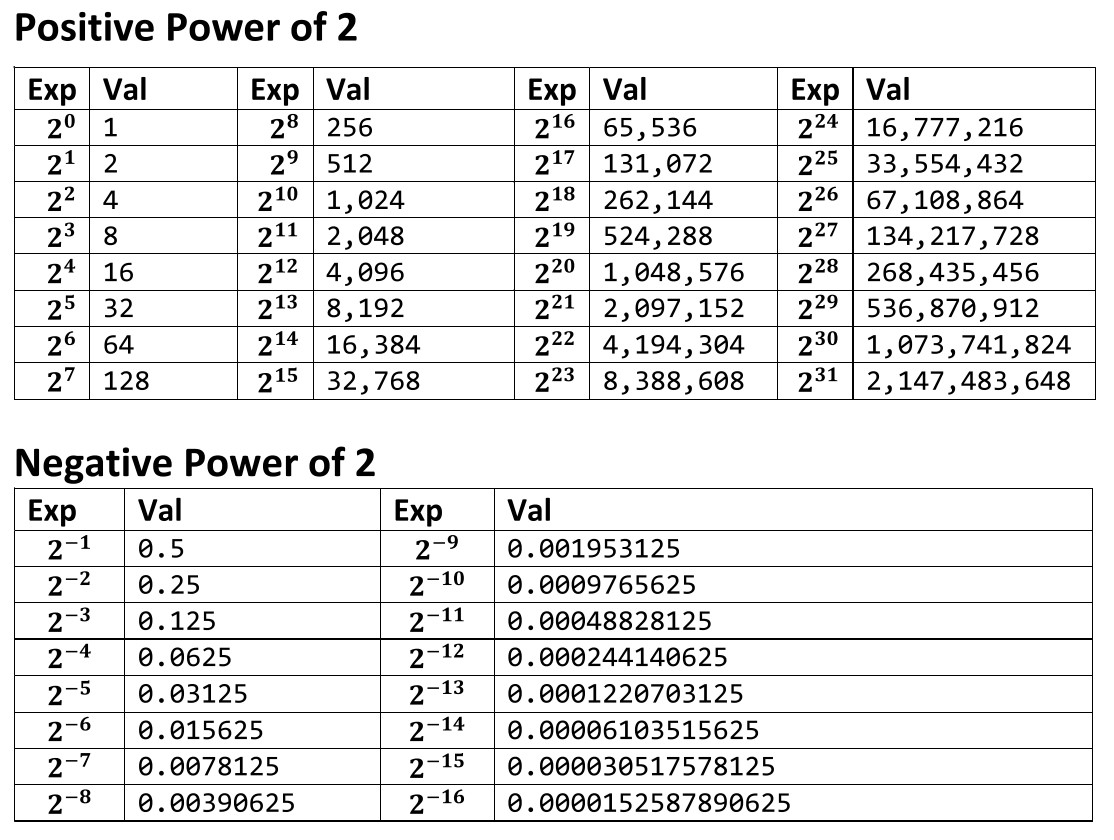
\includegraphics[width=\columnwidth]{powers_of_2.jpg}
\end{center}

\end{multicols*}
\end{document}
